\documentclass[a4paper, 12pt]{article}
\usepackage{graphicx} % Required for inserting images
\usepackage{textcomp}
\usepackage{fullpage}
\usepackage{amsmath}
\usepackage{xcolor}
\usepackage{float}
\usepackage{geometry}
\usepackage{biblatex}
\geometry{margin=1in}
\usepackage{enumitem}
\usepackage{hyperref}
\usepackage{microtype}
\usepackage{gensymb}
\usepackage{parskip}
\hypersetup{
    colorlinks=true,        % Enable colored links
    linkcolor=teal,         % Set color for internal links
    citecolor=teal,         % Set color for citations
    filecolor=teal,         % Set color for file links
    urlcolor=teal           % Set color for URLs
}

\usepackage[version=4]{mhchem}
\title{Chemistry Honors Study Guide}
\author{Semester 1 Final Exam}
\date{Test date: December 17}

\begin{document}

\maketitle

\tableofcontents

\newpage

\section{Study Resources}

\href{https://schoology.santacatalina.org/course/7352977547/materials/gp/7623195638}{Final Exam Study Guide}
\\
\href{https://www.youtube.com/c/TheOrganicChemistryTutor?app=desktop}{The Organic Chemistry Tutor}
\\
\href{https://www.youtube.com/@khanacademy}{Khan Academy}
\\
\href{https://www.youtube.com/watch?v=uVFCOfSuPTo&list=PL8dPuuaLjXtPHzzYuWy6fYEaX9mQQ8oGr}{Crash Course Chemistry}
\\
\href{https://chatgpt.com/}{ChatGPT}
\\
\href{https://chemquiz.net/geo/}{Molecular Geometry \& VSEPR Quiz}

\section{Basic Scientific Concepts}

\subsection{Definitions}

\begin{itemize}[leftmargin=*, nosep]
    \item \textbf{\textit{scientific law:}} A statement describing or predicting natural phenomena.
    \item \textbf{\textit{scientific theory:}} An explanation for natural phenomena.
    \item \textbf{\textit{accuracy:}} A measure of how close measurements are to the true value.
    \item \textbf{\textit{precision:}} A measure of how close measurements are to each other.
    \item \textbf{\textit{physical property:}} A characteristic of a substance that can be observed or measured without altering its identity.
    \item \textbf{\textit{chemical property:}} A characteristic of a substance that can only be observed or measured when a chemical reaction occurs (the substance is converted into a different substance). 
\end{itemize}

\subsection{The Scientific Method}
make an \textbf{observation} $\xrightarrow{}$ ask a \textbf{question} $\xrightarrow{}$ background \textbf{research} $\xrightarrow{}$ form a \textbf{hypothesis} $\xrightarrow{}$ \textbf{test} the hypothesis $\xrightarrow{}$ \textbf{analyze} the data $\xrightarrow{}$ \textbf{communicate} your findings... and repeat!

\subsection{Law v. Theory}
\textbf{Law} is the \textbf{``what"}, while \textbf{theory} is the \textbf{``why"}. Both have been proven but can be disproven and are supported by scientific consensus.  

Example: Newton's First Law, also known as the \textcolor{blue}{law of inertia}, states that an object at rest will remain at rest unless acted upon by an outside force. This is an example of a law because it simply explains what happens (i.e. it is predictive). On the other hand, the theory of \textcolor{blue}{evolution by natural selection} is classified as theory because it is a comprehensive explanation based on an observation.

\subsection{Accuracy v. Precision}
Having both accuracy and precision (see definitions above) is ideal for data collection. Here are some examples of one, both, or neither (where true value = 1.0): 

\textbf{Accurate, but not precise:} 1.17, 1.28, 0.85
\\
\textbf{Precise, but not accurate:} 2.8, 2.75, 2.9
\\
\textbf{Accurate and precise:} 1.1, 1.0, 1.01
\\
\textbf{Neither accurate nor precise:} 6.08, 3.1, 0.5


\subsection{Physical v. Chemical Properties}
(\underline{not an exhaustive list})

\subsubsection{Physical Properties}
\begin{itemize}[leftmargin=*, nosep]
    \item Color
    \item Melting/Boiling point
    \item Density
    \item Solubility
    \item Conductivity
\end{itemize}

\subsubsection{Chemical Properties}
\begin{itemize}[leftmargin=*, nosep]
    \item Reactivity
    \item Smell
    \item Flammability
    \item Toxicity
    \item pH
\end{itemize}

\subsection{Classifying Matter}

\subsubsection{Classifying By Phase}
\textbf{Solid:} holds its shape, not compressible, closely packed, fixed relative positions.
\\
\textbf{Liquid:} conforms to container, not compressible, unfixed relative positions, closely packed.
\\
\textbf{Gas:} conforms to container, compressible, unfixed relative positions, loosely packed.
\\
\textbf{Plasma:} an ionized gas with electrical charge. 

\subsubsection{Classifying By Composition}
\underline{Matter}: \textbf{pure substance} or \textbf{mixture}
\\
\underline{Pure substance:} \textbf{element} \textcolor{blue}{(Au, Ag, Fe, Pb, S$_8$)} or \textbf{compound} \textcolor{blue}{(H$_2$O, NaCO$_3$, CO$_2$, C$_6$H$_{\text{12}}$O$_6$)}
\\
\underline{mixture:} \textbf{homogeneous}, uniformly mixed \textcolor{blue}{(solutions, alloys, dish soap)} or \textbf{heterogeneous}, not uniformly mixed \textcolor{blue}{(oil + water, sand + salt, salad, milk)}

\section{Basic Mathematical Concepts}

\subsection{Significant Digits}
\textbf{Rules for Significant Digits:}
\begin{enumerate}[leftmargin=*, nosep]
    \item All nonzero digits are significant.
    \item Leading zeros (to the left of the first nonzero digit) are never significant.
    \item Trailing zeros are only significant if there is a decimal point.
    \item All zeros between nonzero digits are significant.
\end{enumerate}

\subsection{Scientific Notation}
$$3.14 \times 10^3$$
\\
The first number must be \textbf{$\geq$1} and \textbf{$\leq$10}. When changing a number from scientific notation to standard form (or vice versa), \textbf{the number of significant figures stays the same.}

\subsection{Metric Units}
\begin{center}
\begin{tabular}{c|c|c}
   \textbf{Prefix} & \textbf{Abbreviation} & \textbf{Value} \\\hline
    kilo- & k & 10$^3$ \\
    centi- & c & 10$^{\text{-2}}$ \\
    milli- & m & 10$^{\text{-3}}$ \\
    micro- & $\mu$ & 10$^{\text{-6}}$ \\
    nano- & n & 10$^{\text{-9}}$ \\
\end{tabular}
\end{center}

\subsubsection{Metric Unit Conversions}
Question: How many micrometers are in 456 kilometers? (1 kilometer = 1,000,000,000 micrometers)

$$456 \: km \times \frac{1,000,000,000 \: \mu m}{1 \: km} = 456,000,000,000 \: \mu m$$
\\
\noindent The first number is the number of kilometers there were in the original question; the second is the unit fraction (equal to 1). The original unit ($km$, in this case) should be put at the bottom of the fraction so it cancels out.

\section{The Periodic Table of Elements}

\textcolor{teal}{{\href{https://ptable.com}{Online Periodic Table}}}

\subsection{Definitions}
\begin{itemize}[leftmargin=*, nosep]
    \item \textbf{\textit{Aufbau principle:}} States that electrons first occupy the orbitals with the lowest energy.
    \item \textbf{\textit{isotopes:}} Atoms of the same element (same number of protons) with different atomic masses (different number of neutrons).
    \item \textbf{\textit{Pauli exclusion principle:}} States that no two electrons in the same atom can have the same four quantum numbers.
\end{itemize}

\subsection{Classifications}

\begin{itemize}[leftmargin=*, nosep]
    \item Group 1: \textbf{alkali metals}
    \item Group 2: \textbf{alkali earth metals}
    \item Groups 3-12: \textbf{transition metals}
    \item Group 17: \textbf{halogens}
    \item Group 18: \textbf{noble gases}
\end{itemize}

\subsection{Properties}
\textbf{Metals} are \textbf{good conductors of heat and electricity}, \textbf{malleable}, \textbf{ductile}, and \textbf{shiny}.
\\
\textbf{Nonmetals} are \textbf{insulators} (not conductive) and \textbf{brittle.}
\\
\textbf{Metalloids}, also known as semi-conductors, are \textbf{semi-conductive}.

\subsection{The Atom}\footnote{www.universetoday.com/56469/atom-diagram/\#google\_vignette}

\begin{center}
\begin{tabular}{c|c|c|c}

     \textbf{Name} & \textbf{Mass (amu)} & \textbf{Charge} & \textbf{Location} \\\hline
     proton & 1 & +1 & nucleus \\
     neutron & 1 & 0 & nucleus \\
     electron & negligible & -1 & orbitals 
\end{tabular}
\end{center}

\begin{figure}[H]
    \centering
    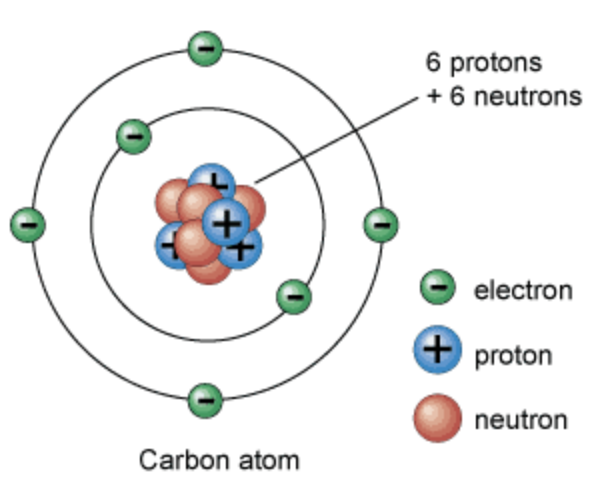
\includegraphics[width=0.5\linewidth]{atom.png}
    \label{fig:lalalalalalalla}
\end{figure}

\subsection{Electron Configuration}
\subsubsection{Full Electron Configuration}
Electrons can exist in 4 types of orbitals: s, p, d, and f. \textbf{s, p, and d} are the only orbitals that will appear on the test. Each orbital can hold a maximum of \textbf{2 electrons.}\footnote{https://madoverchemistry.com/2017/03/14/41-the-periodic-table-spdf-blocks/}

\begin{figure}[H]
    \centering
    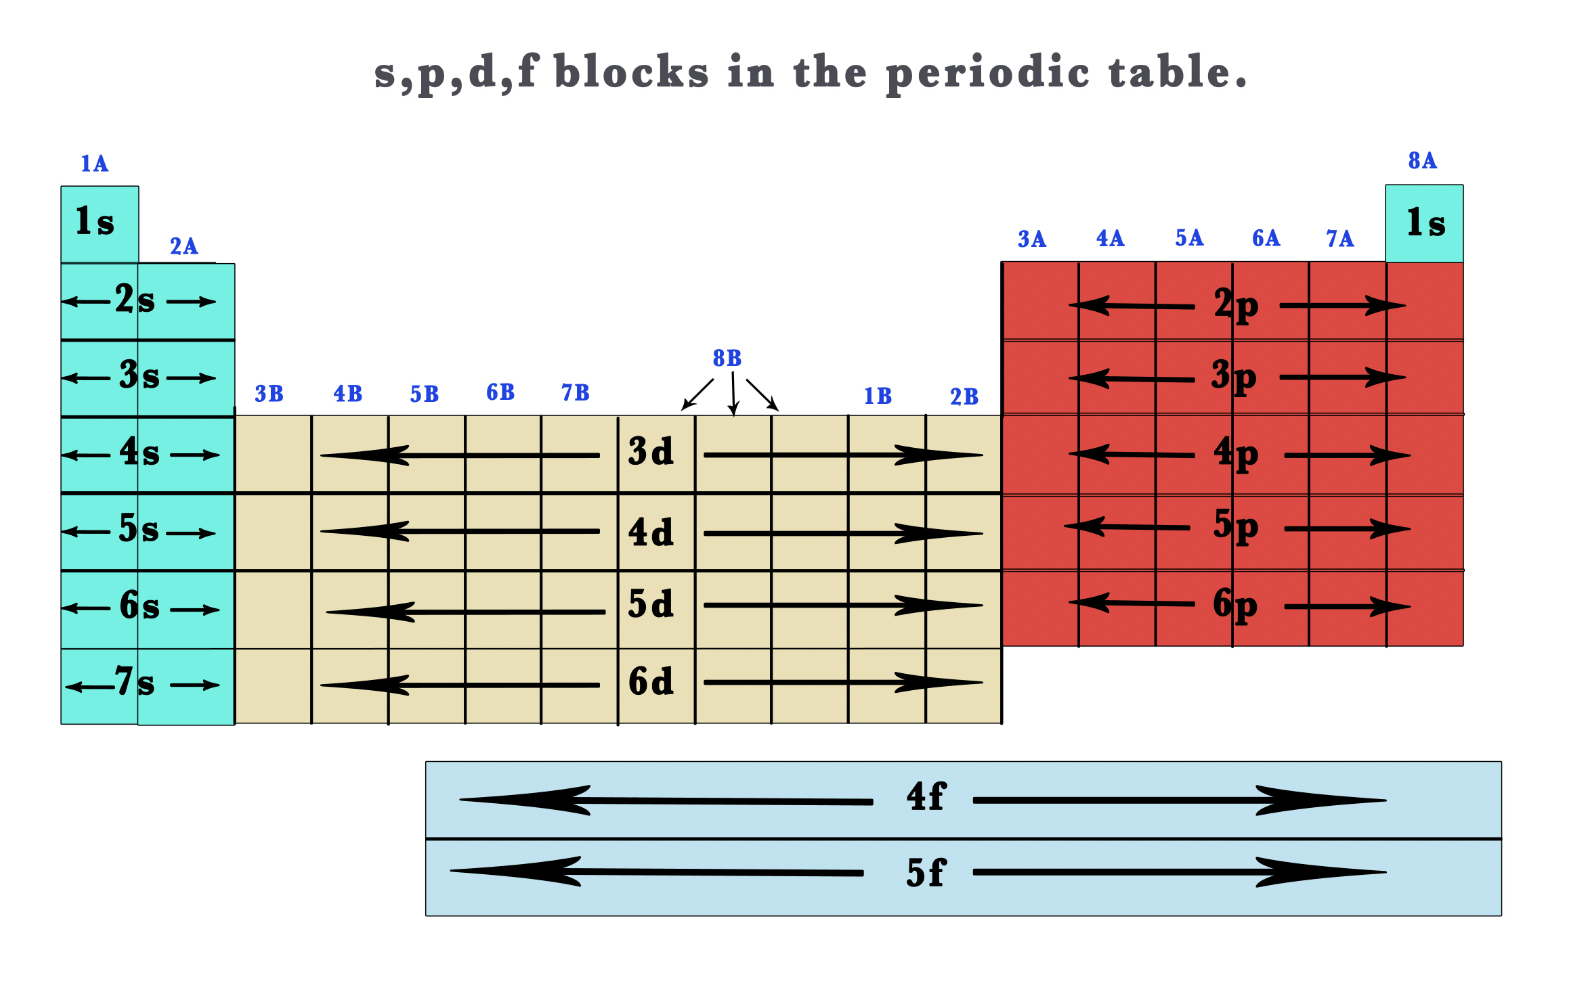
\includegraphics[width=0.6\linewidth]{spdfblocks.png}
    \label{fig:CHEMISTRY}
\end{figure}
\noindent There is/are \textbf{1 $s$ orbital}, \textbf{3 $p$ orbitals}, and \textbf{5 $d$ orbitals\footnote{$d$ orbitals appear only after 4$s$.}} per energy level. More energy levels are added with more rows on the periodic table. The electron configuration is a notation that specifies the energy level, the type of orbital, and the number of electrons in that specific orbital. According to the Aufbau Principle, orbitals are filled in this order: 

\begin{figure}[H]
    \centering
    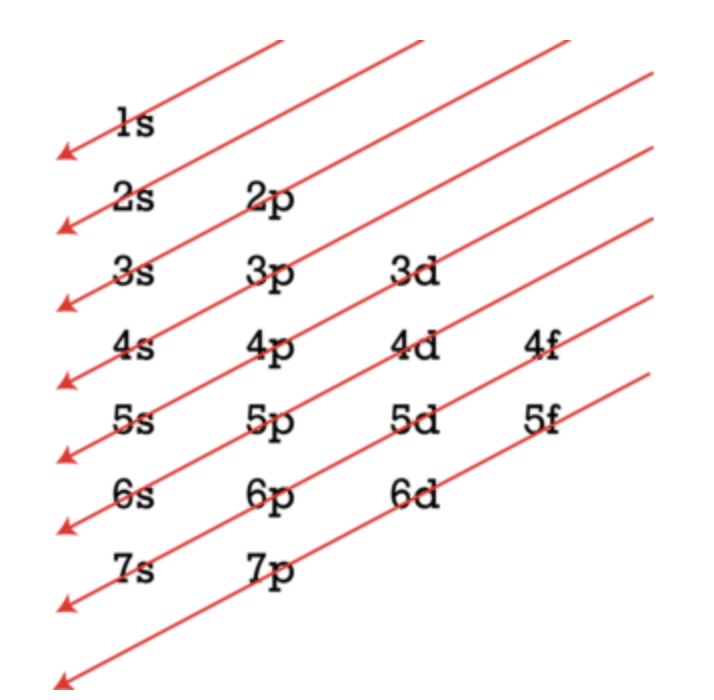
\includegraphics[width=0.4\linewidth]{aufbauprinciple.png}
    \label{fig:please no errors <3}
\end{figure}

\noindent In the following example, the superscript indicates the number of electrons, the letter indicates the orbital type, and the number indicates the energy level.

Example: \textcolor{blue}{Bromine (Br): $1s^22s^22p^63s^23p^5$}

\subsubsection{Noble Gas Configuration}
For noble gas configurations, take the name of the last noble gas, put it in brackets, then write the rest of the configuration, omitting that of the noble gas.

Example: \textcolor{blue}{Bromine (Br): $\text{[Ne]}3s^23p^5$}

\subsection{Electron Box Diagrams}
In electron box diagrams, each box represents an orbital. (The boxes will already be drawn on the test.)

\textbf{Things to remember:}
\begin{itemize}[leftmargin=*, nosep]
    \item Two arrows in the same box should be pointing in different directions (one up, one down).
    \item For multiple orbitals, place an arrow in each orbital first.
\end{itemize}

\begin{figure}[H]
    \centering
    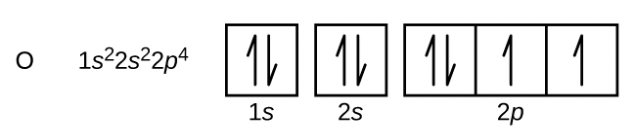
\includegraphics[width=0.5\linewidth]{electronboxdiagrams.png}
    \label{fig:latex hates me}
\end{figure}

\subsection{Ions}
The charge on particles is determined by adding the number of negative charges (adding a negative number) to the number of positive charges.

Example: The charge on an element with 5 protons and 2 electrons is \textcolor{blue}{+3}.

\subsection{Isotopic Symbols}
\ce{^{A}_{B}X} or \ce{^{A}X} or X-A

where:
\begin{itemize}[leftmargin=*, nosep]
    \item X = atomic symbol
    \item A = mass number (protons + neutrons)
    \item B = atomic number
\end{itemize}

\subsection{Quantum Numbers}

\textbf{$n$}, the \textbf{principle quantum number,} indicates the \textbf{orbital shell} in which an electron is in (1, 2, 3, 4, etc.)

\textbf{$l$}, the \textbf{angular quantum number,} indicates the \textbf{orbital type.}
\\
$s$ orbital $\xrightarrow{}$ 0
\\
$p$ orbital $\xrightarrow{}$ 1
\\
$d$ orbital $\xrightarrow{}$ 2

\textbf{$m_l$}, the \textbf{magnetic quantum number,} indicates the specific orbital in which the electron is located. The number of possibilities for $m_l$ correspond to the number of orbitals.
\\
$s$ orbital $\xrightarrow{}$ 0
\\
$p$ orbital $\xrightarrow{}$ -1, 0, 1
\\
$d$ orbital $\xrightarrow{}$ -2, -1, 0, 1, 2

\textbf{$m_s$}, the \textbf{spin quantum number,} indicates the spin on the electron. Electrons in the same orbital have opposite spins. The only two possibilities for this number are +$\frac{1}{2}$ and -$\frac{1}{2}$.

\section{Ionic Compounds}

\subsection{Definitions}
\begin{itemize}[leftmargin=*,nosep]
\item \textbf{\emph{ion:}} Charged particle.
\item \textbf{\emph{cation:}} Positively charged particle. All cations are metals.
\item \textbf{\emph{anion:}} Negatively charged particle. All anions are either nonmetals or metalloids.
\item \textbf{\emph{ionic compound:}} Created from electrostatic attraction between cations and anions.
\item \textbf{\emph{salt:}} Another name for an ionic compound.
\item \textbf{\emph{Type I cation:}} Includes groups 1, 2, 13, Ag$^+$, Zn$^{\text{2+}}$. Can only have a single charge state.
\item \textbf{\emph{Type II cation:}} Transition metals (not Ag or Zn), Pb, Sn. Can have multiple charge states.
\end{itemize}

\subsection{Ionic Bonding}
Atoms form bonds to fill their valence shells. Depending on what is easier for an atom of each element (getting rid of/gaining electrons), they will have a positive or negative charge.

Once bonded, the charges on each ion must cancel out. Like fraction addition, we change the charges to their least common multiple (if they are not already equal).

Example: \textcolor{blue}{2K$^{\text{1+}}$ + O$^{\text{2-}}$ $\xrightarrow{}$ K$_2$O} \textbf{cation first!}

After the bonding occurs, the charge on the resulting particle is neutral.

\subsection{Naming Compounds with Type I Cations (Monatomic Anions)}
\fbox {\textcolor{blue}{\textbf{name of cation + anion ending in -ide}}}

Example: \textcolor{blue}{Al$_2$S$_3$: Aluminum sulfide} 
Note that the number of atoms present does not influence the naming.

\subsection{Naming Compounds with Type II Cations (Monatomic Anions)}
\fbox {\textcolor{blue}{\textbf{cation + charge on cation + anion ending in -ide}}}

Example: \textcolor{blue}{Fe$_2$O$_3$: iron (III) oxide}

In this example, the number of iron atoms does not matter; the number in parentheses is always the charge.

\subsection{Naming Compounds with Polyatomic Anions}
\begin{itemize}[leftmargin=*,nosep]
    \item NO$_3$$^-$: \textbf{nitrate}
    \item ClO$_3$$^-$: \textbf{chlorate}
    \item CO$_3$$^{2-}$: \textbf{carbonate}
    \item SO$_4$$^{2-}$: \textbf{sulfate}
    \item PO$_4$$^{3-}$: \textbf{phosphate}
\end{itemize}
|||||||||||||||||||||||||||||||||||

\noindent \textbf{\underline{N}\textcolor{red}{i}ck the \underline{C}\textcolor{red}{a}m\textcolor{red}{e}l ate \underline{Cl}\textcolor{red}{a}m \underline{S}\textcolor{red}{u}pp\textcolor{red}{e}r in \underline{P}h\textcolor{red}{oe}n\textcolor{red}{i}x}

\textbf{Number of consonants:} Number of oxygen atoms
\\
\textbf{\textcolor{red}{Number of vowels:}} Number of negative charges

\noindent |||||||||||||||||||||||||||||||||||
\begin{table}[ht]
    \centering
    \begin{tabular}{c|c|c|c}
         \textbf{Relative \# of Oxygen } & \textbf{Prefix/suffix} & \textbf{Equation} & \textbf{Name} \\\hline
        +1 & per...ate & ClO$_4$$^-$ & perchlorate \\
        -1 & -ite & ClO$_2$$^-$ & chlorite \\
        0 & -ate & ClO$_3$$^-$ & chlorate \\
        -2 & hypo...ite & ClO$^-$ & hypochlorite
    \end{tabular}
    \label{tab:my_label}
\end{table}

\noindent Example: \textcolor{blue}{PO$_5$$^{\text{3-}}$ = perphosphate}; \textcolor{blue}{Na$_3$PO$_5$ = sodium perphosphate}

(Note that the charge does not change with the number of oxygen atoms, but when the polyatomic anion bonds with a cation, the resulting compound becomes neutral.)

\section{Covalent Compounds}

\subsection{Definitions}
\begin{itemize}[leftmargin=*,nosep]
    \item \textbf{\emph{covalent compound:}} A compound bonded covalently (sharing valence electrons).
\end{itemize}

\subsection{Naming Binary Covalent Compounds (two elements)}
\fbox {\textbf{\textcolor{blue}{if $>$ 1, number prefix + first element + number prefix + second element + -ide}}} %fix this part

Example: \textcolor{blue}{N$_2$O$_3$: \textbf{di}nitrogen \textbf{tri}oxide}

\textbf{Prefixes:}
\begin{enumerate}[leftmargin=*,nosep]
    \item \textbf{mono}-
    \item \textbf{di}-
    \item \textbf{tri}-
    \item \textbf{tetra}-
    \item \textbf{penta}-
    \item \textbf{hexa}-
    \item \textbf{hepta}-
    \item \textbf{octa}-
\end{enumerate}

\section{Identification and Diagrams}

\subsection{Definitions}

\begin{itemize}[leftmargin=*, nosep]
\item \textbf{\textit{resonance:}} The sharing of electrons between multiple bonds, esp. in polyatomic ions.
\end{itemize}

\subsection{Identifying Ionic vs Covalent Compounds}

\textbf{Ionic compounds...}
\begin{itemize}[leftmargin=*,nosep]
    \item start with a \textbf{metal} or with \textbf{NH$_4$$^+$} (ammonium).
    \item form from the electrostatic attraction of \textbf{metals with nonmetals/metalloids}.
\end{itemize}

\textbf{Covalent compounds...}
\begin{itemize}[leftmargin=*,nosep]
    \item are formed between \textbf{metals or metalloids}.
    \item involve the \textbf{sharing of electrons}.
\end{itemize}

\subsection{Lattice Diagrams}

\textbf{Essential aspects of lattice diagrams:}
\begin{itemize}[leftmargin=*,nosep]
    \item separated charges (- not touching +)
    \item atomic ratio
    \item atomic symbol
    \item at least 2 repetitions
\end{itemize}

\subsubsection{Identifying Covalent Lattice Diagrams}
\textbf{Molecular:} distinct molecules, not interconnected (such as H$_2$O)
\\
\textbf{Network:} interconnected network of atoms (such as C (diamond))

\subsubsection{Ionic Lattice Diagrams}

Example: \textcolor{blue}{NaCl (sodium chloride/table salt)}\footnote{https://www.elevise.co.uk/gac2c.html}

\begin{figure}[ht]
    \centering
    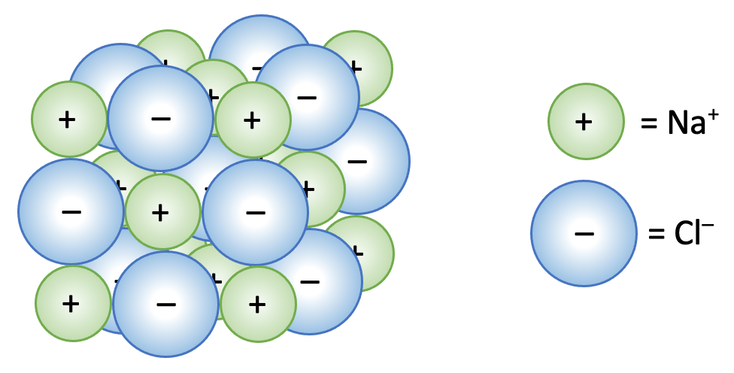
\includegraphics[width=0.5\linewidth]{lattice.png} 
    \label{fig:1}
\end{figure} 

\subsubsection{Metallic Lattice Diagrams}

\begin{figure}[ht]
    \centering
    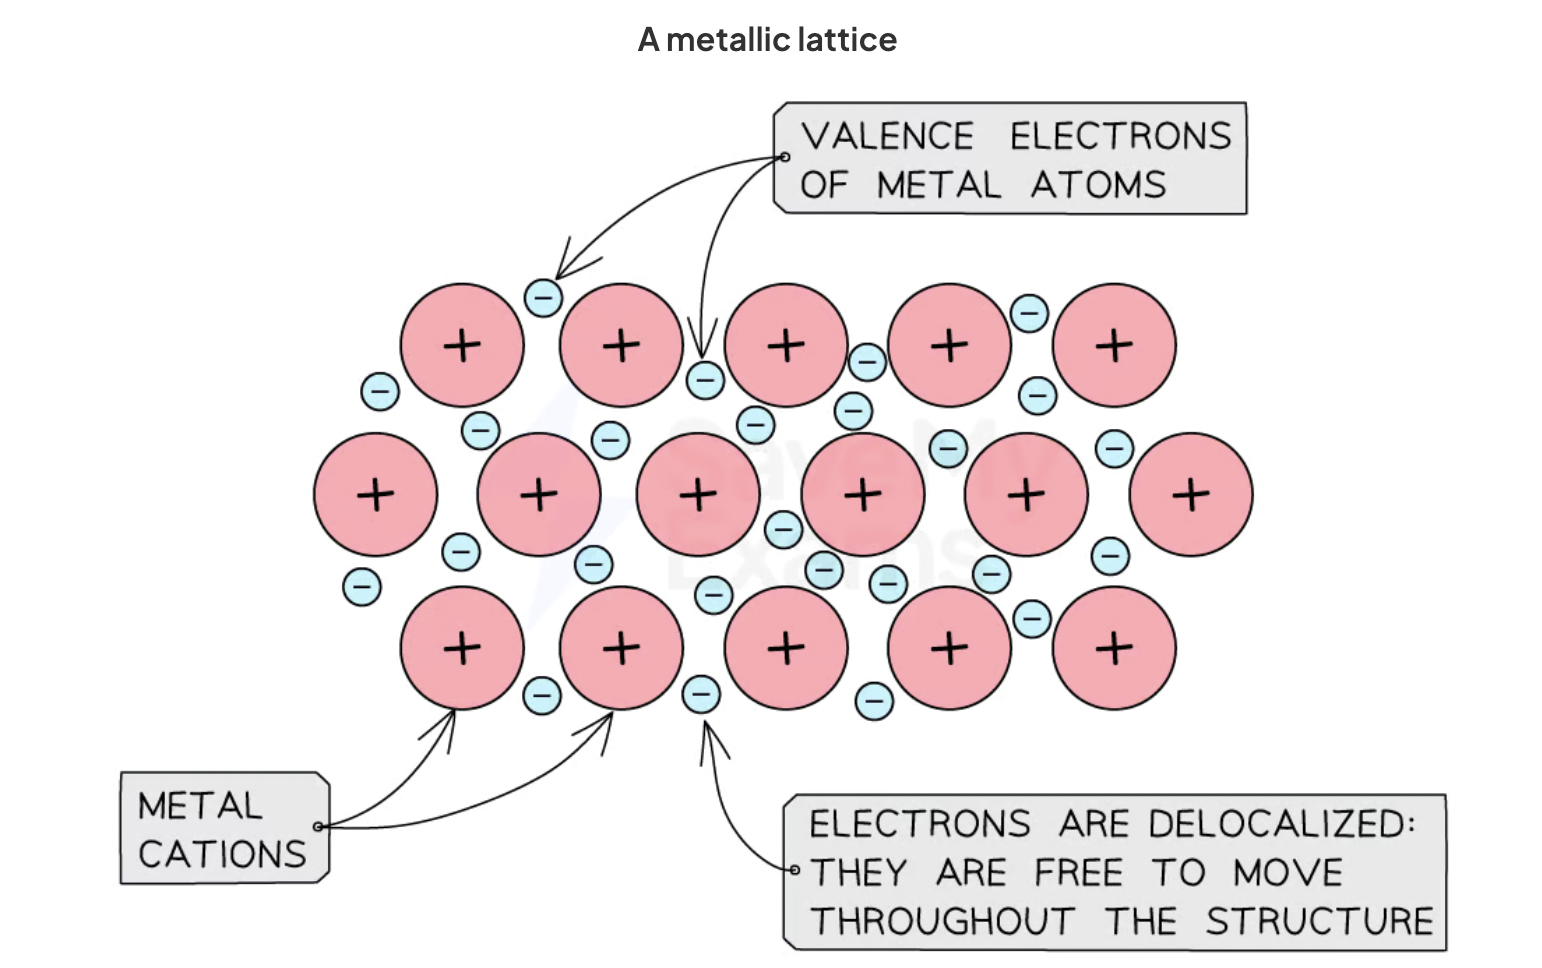
\includegraphics[width=0.5\linewidth]{metalliclattice.png}
    \label{fig:1.3?}
\end{figure}
\noindent (This is the diagram for all metallic bonding. The number of atoms, electrons, and arrow directions do not matter as long as the picture shows a cluster of atoms with moving electrons.)\footnote{https://www.savemyexams.com/ap/chemistry/college-board/22/revision-notes/unit-2-molecular-and-ionic-compound-structure-and-properties/2-4-structure-of-metals-and-alloys/representing-metallic-bonding/}

\subsection{Lewis Dot Structures}

\subsubsection{Atomic LDS}

\begin{figure}[H] 
    \centering
    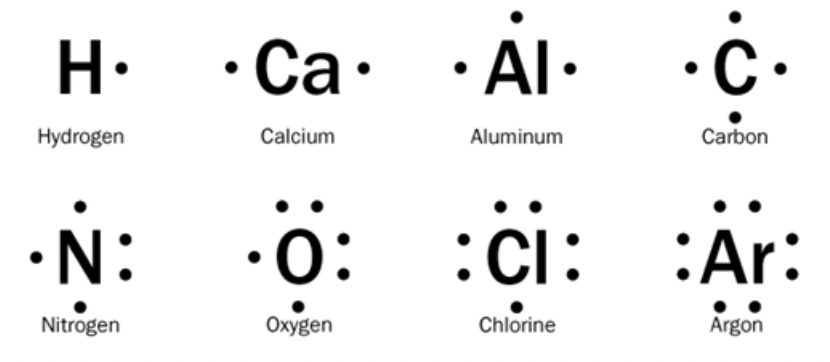
\includegraphics[width=0.5\linewidth]{atomiclds.png}
    \label{fig:2}
\end{figure} 
\noindent As shown above, the number of valence electrons increases as you go across the periodic table, so the number of dots increase. (Placement is intentional -- when drawing the atomic structures, electrons are separated, but in ionic/covalent structures, electrons are drawn in pairs.)\footnote{https://americanboard.org/Subjects/general-science/bonding-and-atomic-structure/}

\subsubsection{Ionic LDS}
\begin{itemize}[leftmargin=*,nosep]
    \item The \textbf{cation} always has an \textbf{empty valence shell} (no dots).
    \item The \textbf{anion} always has a \textbf{filled valence shell} with \textbf{brackets} around the atom.
    \item \textbf{Charges should be indicated} in the top right of each atom.
    \item Charges are \textbf{properly separated.}
\end{itemize}

\noindent Example: \textcolor{blue}{MgO (magnesium oxide)}\footnote{https://scienceready.com.au/pages/lewis-dot-diagram}

\begin{figure}[H]
    \centering
    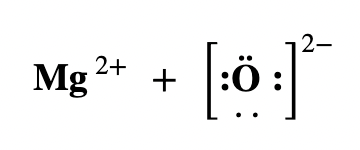
\includegraphics[width=0.5\linewidth]{ioniclds.png}
    \label{fig:2.5}
\end{figure}

\subsubsection{Covalent LDS}
\begin{enumerate}[leftmargin=*,nosep]
    \item Determine the \textbf{number of valence electrons.}
    \item Determine the \textbf{central atom} if there are more than 2 atoms. \textbf{The central atom (with the exception of hydrogen) should be the one with the lowest electronegativity.}
    \item \textbf{Draw the LDS} so that \textbf{each atom (note exceptions below) has a full valence shell.}
    \item Replace shared electrons with lines. \textbf{(2 electrons = 1 bond = 1 line).}
\end{enumerate}

\begin{figure}[H]
    \centering
    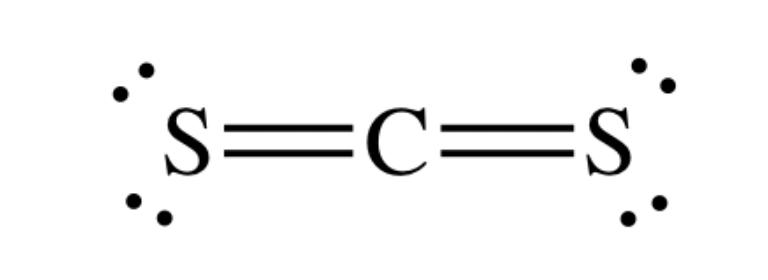
\includegraphics[width=0.3\linewidth]{covalentlds.png}
    \label{fig:3}
\end{figure}

\subsubsection{Exceptions}
\begin{itemize}[leftmargin=*,nosep]
    \item \textbf{Hydrogen} forms a \textbf{full duet} (2 valence electrons).
    \item \textbf{Boron} forms a \textbf{full sestet} (6 valence electrons).
    \item Elements in the \textbf{third period or below} may have an \textbf{expanded octet} (more than 8 electrons in their valence shell).
\end{itemize}

\noindent Example: \textcolor{blue}{PCl$_5$ (phosphorus pentachloride)}\footnote{https://www.fishersci.ca/shop/products/phosphorus-v-chloride-98-thermo-scientific/p-3257053}

\begin{figure}[H]
    \centering
    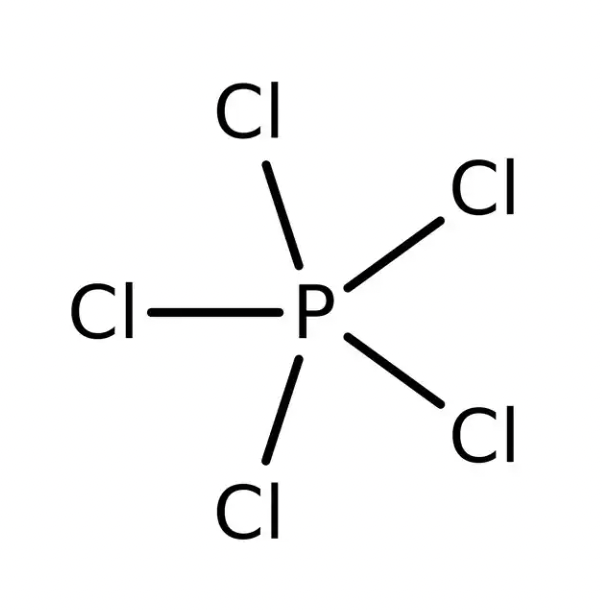
\includegraphics[width=0.2\linewidth]{exceptionlds.png}
    \label{fig:4}
\end{figure}



\subsubsection{Resonance LDS}
There are many possible resonance structures of one polyatomic anion depending on the number of double bonds.

Example: \textcolor{blue}{CO$_3$$^{\text{2-}}$ (carbonate)}\footnote{https://kpu.pressbooks.pub/organicchemistry/chapter/1-3-resonance-structures/}

\begin{figure}[H]
    \centering
    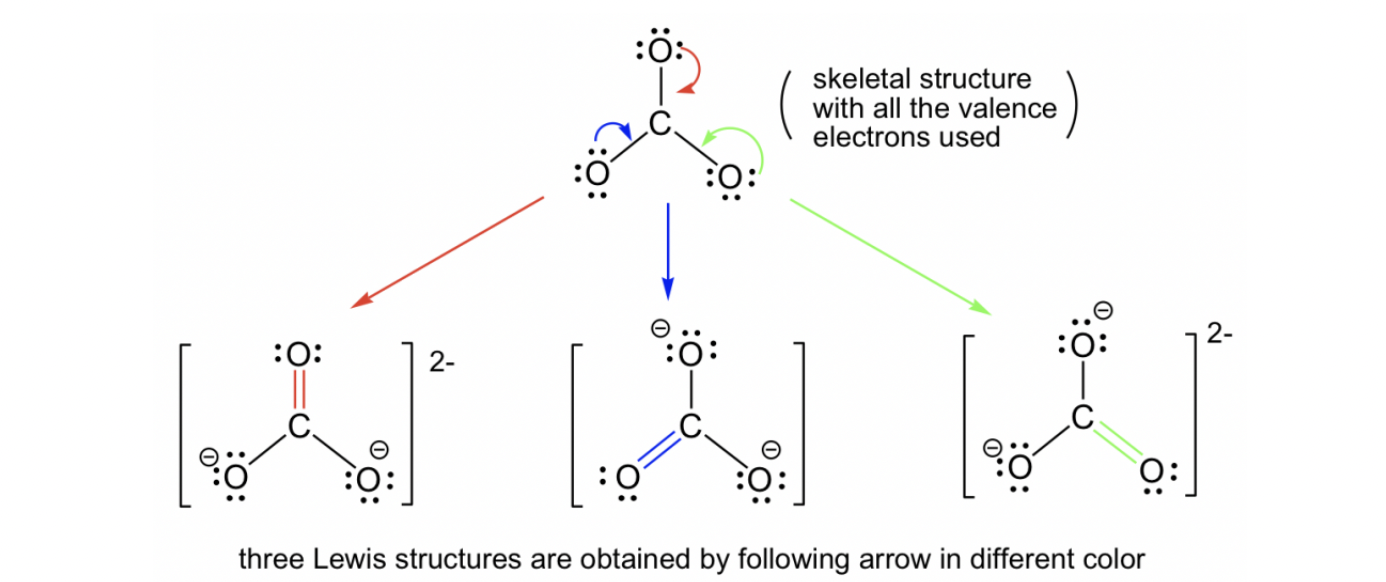
\includegraphics[width=0.8\linewidth]{resonancelds.png}
    \label{fig:200?!}
\end{figure}

\noindent This diagram shows the possibilities of where the double bond could be in carbonate.


\subsubsection{Combined Resonance LDS}
In a polyatomic ion, when the central atom has a formal charge of 0, the oxygen atoms around it share their remaining formal charges. A dotted line instead of a bond is drawn from each oxygen atom to the central atom to indicate the shared charge.\footnote{https://chemfiesta.org/2015/09/18/resonance-structures/}

Example: \textcolor{blue}{NO$_2$$^-$ (nitrite)}

\begin{figure}[H]
    \centering
    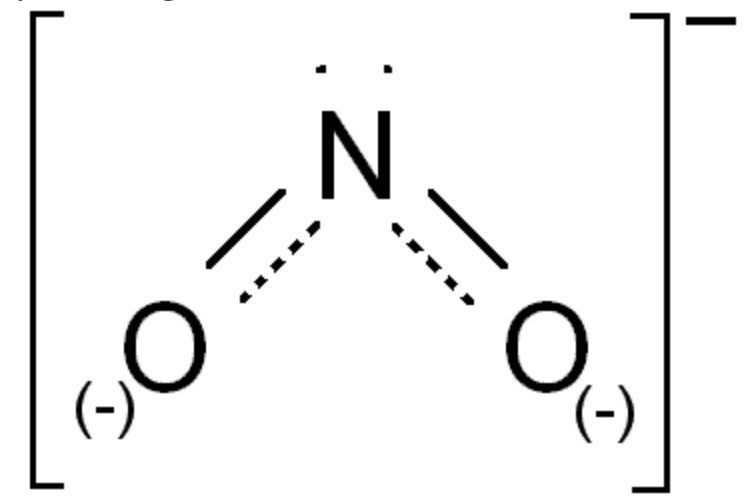
\includegraphics[width=0.3\linewidth]{combinedresonance.png}
    \label{fig:something???}
\end{figure}

\subsubsection{Polyatomic Ions}
Polyatomic ions are \textit{covalent structures within an ionic structure.} Draw the Lewis dot structure of a polyatomic ion as a covalent compound, treating it as a single unit, then add the element it bonds ionically with to the diagram. As usual, include brackets when necessary.

When making LDS with polyatomic ions that have expanded octets, the \textbf{formal charge on the central atom must equal 0.} The formula to find formal charge of an atom is as follows: 
 $$ \text{formal charge = \# of valence electrons} - \text{\# of lone pair electrons} - \text{\# of bonds} $$

\noindent Note that the number of lone pair electrons refers to the number of individual electrons, not the number of lone pairs. (Formal charge does not need to be indicated unless the problem states otherwise.)

\begin{figure}[H]
    \centering
    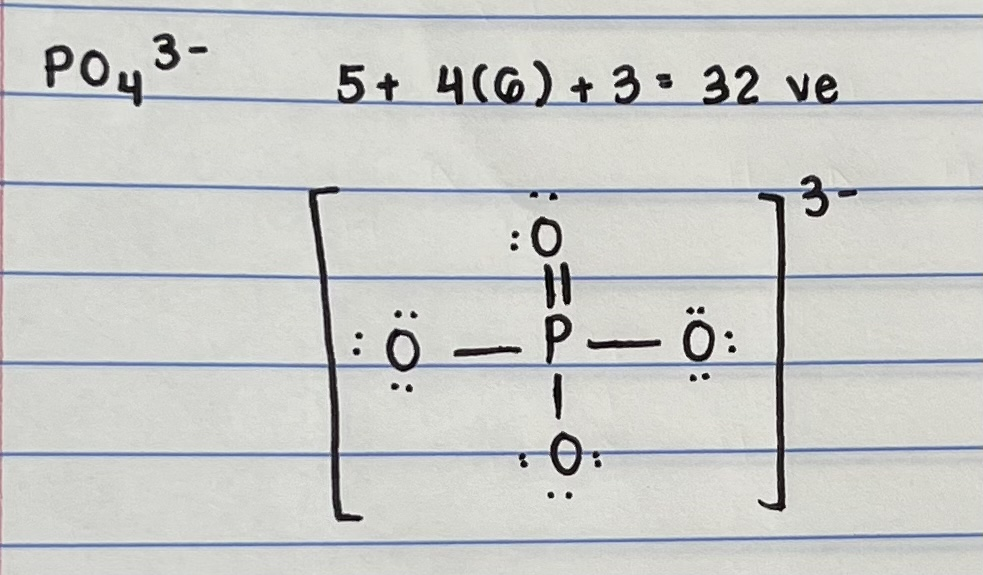
\includegraphics[width=0.5\linewidth]{expandedlds.jpeg}
    \label{fig:bunnies are cute}
\end{figure}
\noindent Example: \textcolor{blue}{PO$_4$$^{3-}$ (phosphate)}

\section{Periodic Table Trends}

\subsection{Definitions}
\begin{itemize}[leftmargin=*, nosep]
    \item \textbf{\textit{effective nuclear charge:}} The force felt by an electron from the nucleus.
    \item \textbf{\textit{electronegativity:}} The tendency of an atom to attract electrons.
    \item \textbf{\textit{ionization energy:}} The energy it takes to remove an electron from an atom.
    \item \textbf{\textit{atomic radius:}} The size of the atom, or, more precisely, the distance from an atom's nucleus to its outermost orbital.
\end{itemize}

\subsection{Coulomb's Law}

$$F = k\frac{q_1q_2}{r^2}$$

where:
\begin{itemize}[nosep]
    \item $F$ = force felt by electron
    \item $k$ = Coulomb's constant (not important for this test)
    \item $q_1$ = charge on valence electron
    \item $q_2$ = charge on nucleus
    \item $r$ = distance (nucleus to electron)
\end{itemize}

\subsection{Electronegativity and Ionization Energy}
Electronegativity and ionization energy \textbf{increase} as you go \textbf{higher} and to the \textbf{right} in the periodic table.

Electronegativity increases near the top of the periodic table because the distance from the potential electron and the nucleus is smaller (as described by Coulomb's Law above.) Near the right, electronegativity increases because the atoms grow increasingly close to filling their valence shells, needing to attract extra electrons.

Ionization energy increases near the top because it is harder to remove an electron close to the nucleus (again, as described by Coulomb's Law). Near the right, ionization energy increases because it becomes increasingly difficult to remove electrons from atoms that are close to filling their valence shells.

\subsection{Atomic Radii}
The atomic radius \textbf{increases} as you go \textbf{lower} and to the \textbf{left} in the periodic table. This is because as the number of protons increases (as you go to the right), it will pull the electrons closer, resulting in a smaller atomic radius, and as the number of orbitals increases (as you go lower), the atomic radius increases likewise.

\section{Bonding Theories and Geometry}

\subsection{Definitions}
\begin{itemize}[leftmargin=*, nosep]
    \item \textbf{\textit{molecular orbital:}} An orbital that applies to the entire molecule.
    \item \textbf{\textit{electron domain:}} A distinct region around an atom where lone pair electrons/bonds are found.
    \item \textbf{\textit{pi ($\pi$) bond:}} A type of covalent bond that is a combination of two atomic orbitals overlapping laterally.
    \item \textbf{\textit{sigma ($\sigma$) bond:}} A type of covalent bond that is a combination of two atomic orbitals from end to end. There is exactly one $\sigma$ bond in each single, double, and triple bond (the rest are $\pi$ bonds).
    \item \textbf{\textit{VSEPR (ves-per) theory:}} A model predicting the geometric shape of molecules; stands for \textbf{\underline{V}alence \underline{S}hell \underline{E}lectron \underline{P}air \underline{R}epulsion.}
    \item \textbf{\textit{hybridization:}} The combination of two atomic orbitals to create a new type of hybrid orbital.

\end{itemize}

\subsection{Molecular Orbitals}

\subsubsection{$\pi$ Bonding}

\begin{center}
    Two $p$ orbitals overlap laterally \footnote{https://byjus.com/chemistry/sigma-and-pi-bond/}
\end{center}

\begin{figure}[H]
    \centering
    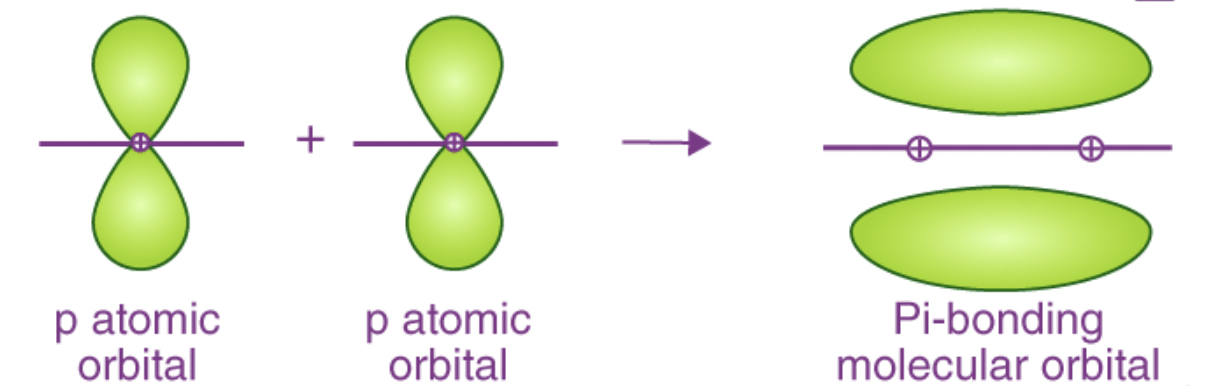
\includegraphics[width=0.5\linewidth]{pibond.png}
    \label{fig:ahhsfhafhshahahdfhoasdf}
\end{figure}

\subsubsection{$\sigma$ Bonding}

\begin{center}
    $s$-$s$ overlap (2 half-filled $s$ orbitals)\footnote{https://www.chemistrylearner.com/sigma-and-pi-bonds.html}
\end{center}

\begin{figure}[H]
    \centering
    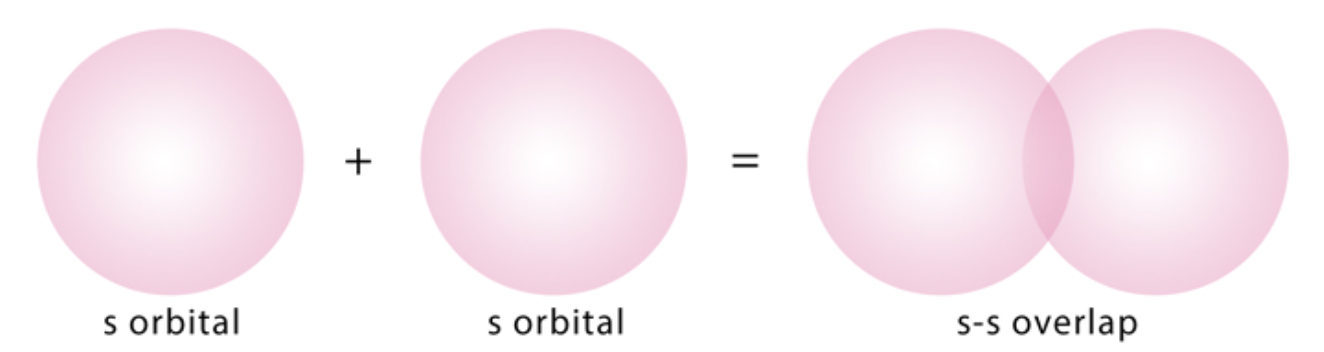
\includegraphics[width=0.45\linewidth]{ssoverlap.png}
    \label{fig:aaaaaaaaaaaaaaaaa}
\end{figure}

\begin{center}
    $s$-$p$ overlap (1 half-filled $s$ orbital and 1 half-filled $p$ orbital)
\end{center}

\begin{figure}[H]
    \centering
    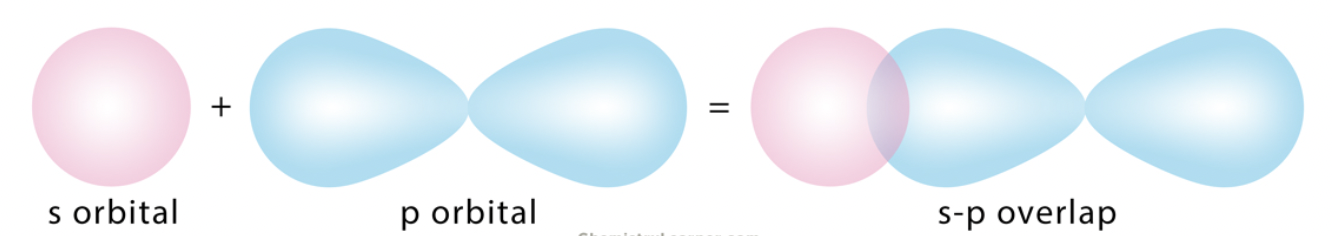
\includegraphics[width=0.5\linewidth]{spoverlap.png}
    \label{fig:enter-label}
\end{figure}

\begin{center}
    $p$-$p$ overlap (2 half-filled $p$ orbitals)
\end{center}

\begin{figure}[H]
    \centering
    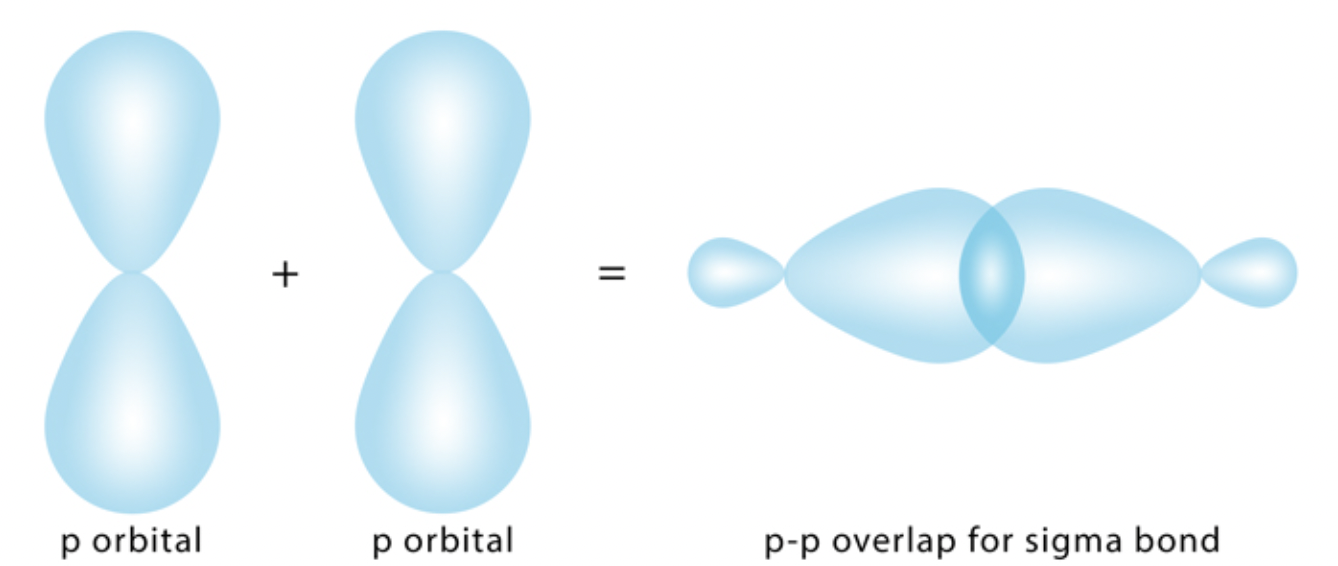
\includegraphics[width=0.45\linewidth]{ppoverlap.png}
    \label{fig:erm}
\end{figure}

\subsection{Drawing a 3-D Molecule}

\begin{itemize}[leftmargin=*, nosep]
    \item line = bond on the plane
    \item 3 lines = bond into the plane
    \item triangle = bond out of the plane \footnote{https://oehha.ca.gov/chemicals/methanol}
\end{itemize}

\begin{figure}[H]
    \centering
    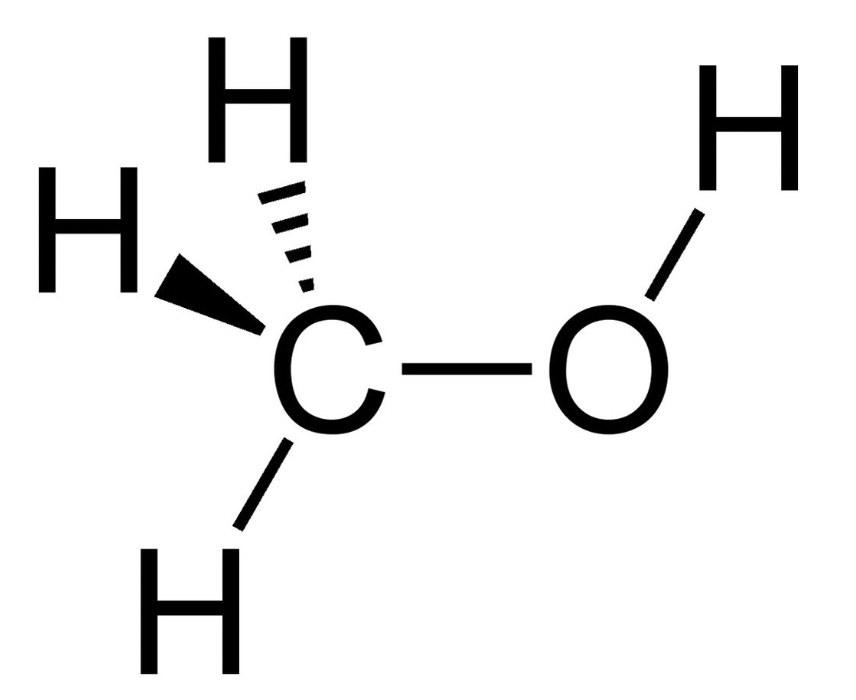
\includegraphics[width=0.3\linewidth]{3dmol.png}
    \label{fig:312456738r902po3iu4}
\end{figure}

\subsection{VSEPR Theory}
(ed = electron domains; lp = lone pair(s))
\subsubsection{Electron Geometry}

\begin{centering}

\begin{tabular}{c|c}
    \textbf{\# ed} & \textbf{Name} \\\hline
    2 & \textit{linear} \\
    3 & \textit{trigonal planar} \\
    4 & \textit{tetrahedral} \\
    5 & \textit{trigonal bipyramidal} \\
    6 & \textit{octahedral}
\end{tabular}

\end{centering}

\subsubsection{Molecular Geometry}
\begin{centering}

\begin{tabular}{c|c|c|c|c|c}
    \textbf{\# ed} & \textbf{0 lp} & \textbf{1 lp} & \textbf{2 lp} & \textbf{3 lp} & \textbf{4 lp} \\\hline
    2 & \textit{linear} & n/a & n/a & n/a & n/a \\
    3 & \textit{trigonal planar} & \textit{bent} & n/a & n/a & n/a \\
    4 & \textit{tetrahedral} & \textit{trigonal pyramidal} & \textit{bent} & n/a & n/a \\
    5 & \textit{trigonal bipyramidal} & \textit{seesaw} & \textit{t-shaped} & \textit{linear} & n/a \\
    6 & \textit{octahedral} & \textit{square pyramidal} & \textit{square planar} & \textit{t-shaped} & \textit{linear}
\end{tabular}

\end{centering}

\subsection{Hybridization}
(The numbers before the orbital type are the number of that orbital type there are, not the energy level.)

$1(s) + 3(p) \xrightarrow{} 4(sp^3)$ (\textbf{tetrahedral} e$^-$ geometry)
\\
$1(s) + 3(p) \xrightarrow{} 3(sp^2) + 1(p)$ (\textbf{trigonal planar} e$^-$ geometry)
\\
$1(s) + 3(p) \xrightarrow{} 2(sp) + 2(p)$ (\textbf{linear} e$^-$ geometry)

\section{Polarity}

\subsection{Definitions}

\begin{itemize}[leftmargin=*, nosep]
    \item \textbf{\textit{polarity:}} Occurs when one atom attracts electron cloud more than another, therefore making one end more negative.
    \item \textbf{\textit{dipole:}} A pair of separated equal and opposite electric charges.
\end{itemize}

\subsection{Bond Polarity by Electronegativity}
Polarity is determined by the following equation:

$$\Delta EN = |EN_1 - EN_2| $$

\begin{itemize}[leftmargin=*, nosep]
\item \noindent If $\Delta EN \leq$ 0.4, the particle is \textbf{nonpolar covalent.}
\item If 0.4 $< \Delta EN \leq$ 1.0, the particle is \textbf{moderately polar covalent.}
\item If 1.0 $< \Delta EN \leq$ 2.0, the particle is \textbf{highly polar covalent.}
\item If $< \Delta EN \geq$ 2.0, the particle is \textbf{ionic.}
\end{itemize}

\subsection{Molecular Polarity}

\begin{itemize}[leftmargin=*, nosep]
    \item If a molecule has no polar bonds, it is not polar.
    \item If a molecule is symmetrical with the same polarity in each bond, it is not polar. (Molecules with linear, trigonal planar, tetrahedral, trigonal bipyramidal, and octahedral molecular geometry and the same element around the central atom are not polar.)
    \item If a molecule contains (a) more electronegative atom(s) on one end than another, the polarity arrow goes in the direction of the electronegative end.
\end{itemize}

\section{Intermolecular Forces (IMFs)}

\subsection{IMF Types (weakest to strongest)}

\subsubsection{London Dispersion Forces (LDFs)}
Occur between all molecules. Only IMF between nonpolar molecules

\begin{itemize}[leftmargin=*, nosep]
    \item weakest IMF
    \item attractions between instantaneous dipoles due to moving electrons
    \item also induced dipoles
    \item $\uparrow$ molecule size, polarizability = $\uparrow$ LDF
\end{itemize}

\subsubsection{Dipole-Dipole Forces (Dip-Dip)}
Formed between polar molecules due to attraction between opposite permanent poles
\textbf{Dipole notation:\footnote{https://byjus.com/chemistry/dipole-moment/}} $\delta^+$ on positive end(s); $\delta^-$ on negative end(s)

\begin{figure}[H]
    \centering
    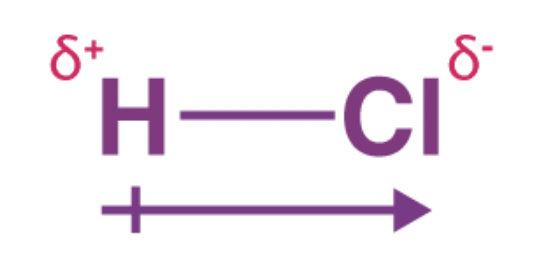
\includegraphics[width=0.3\linewidth]{polarmol.png}
    \label{fig:ummmmmm}
\end{figure}

\subsubsection{Hydrogen ``Bonding" (H-Bonding)}
Occurs between molecules with N---H, F---H, and O---H bonds. A type of dipole-dipole interaction.

\subsubsection{Ion-Dipole Interactions}
Formed between ionic compounds and polar compounds.
$$NaCl_{(s)} \longrightarrow Na^+_{(aq)} + Cl^-_{(aq)}$$
Adding salt to water creates a cage effect, increasing density, because molecules are more tightly packed together due to stronger bonds. In order for ionic compounds to dissolve, ion-dipole forces must be stronger than ionic and H bonds.

\subsection{Macro Effects of IMFs}
$\uparrow$ IMFs = $\uparrow$ boiling point, melting point, surface tension, viscosity

\begin{centering}

\begin{tabular}{c|c|c|c}
    \textbf{Name} & \textbf{Formula} & \textbf{Strongest IMF} & \textbf{Boiling Point} \\\hline
    Water & H$_2$O & H-bonds & 100\degree C \\
    Methane & CH$_4$ & LDFs & -162\degree C \\
    Formaldehyde & CH$_2$O & Dip-dip & -19\degree C \\
    Propane & C$_3$H$_8$ & LDFs & -19\degree C \\
    Hexane & C$_6$H$_{14}$ & LDFs & 68\degree C
\end{tabular}

\end{centering}

\subsubsection{Trends}
\begin{itemize}[leftmargin=*, nosep]
    \item The relative boiling points of molecules of similar sizes depend on the IMFs present. ($\uparrow$ force = $\uparrow$ b.p.)
    \item The relative boiling points of molecules with the same IMFs depend on the sizes of the molecules. ($\uparrow$ size = $\uparrow$ polarizability = $\uparrow$ b.p.)
\end{itemize}

\subsubsection{Miscibility}
\textbf{``Like dissolves like"} --- polar + polar and nonpolar + nonpolar are miscible and create a homogeneous mixture; nonpolar + polar are not miscible and create a heterogeneous mixture

\section{Atoms, Molecules, Moles, Grams}

\subsection{Definitions}

\begin{itemize}[leftmargin=*, nosep]
    \item \textbf{\textit{mole:}} A unit of quantification; 6.02 x 10$^{23}$ (Avogadro's number).
    \item \textbf{\textit{molar mass:}} How many grams a mole of an atom/compound weighs. Units are g/mol.
    \item \textbf{\textit{empirical formula:}} A molecular formula reduced to its lowest ratio of atoms.
\end{itemize}

\subsection{Conversions}

Example: How many \textcolor{blue}{atoms} are in \textcolor{blue}{17 grams} of \textcolor{blue}{MgCl$_2$}?

\textcolor{blue}{\textbf{Step 1:} Draw a conversion map.} In order to get from grams to atoms, the steps are as follows: 
\\
$$g \longrightarrow mol \longrightarrow {\text{molecules}} \longrightarrow {\text{atoms}}$$
\\
\textcolor{blue}{\textbf{Step 2:} Set up the conversion.} Multiply by the conversion factor(s), (a) unit fraction(s) (equal to 1). Set it up so that the same units cancel out in order to get the desired unit in the end.
\\
$$(17\: g) \times \left(\frac{1 \: mol}{95.211 \: g}\right) \times \left(\frac{6.02 \times 10^{23} \: {\text{molecules}}}{1 \: mol}\right) \times \left(\frac{3 \: {\text{atoms}}}{1 \: {\text{molecules}}}\right)$$
\\
\textcolor{blue}{\textbf{Step 4:} Calculate.} 
\\
$$ = \boxed{3.225 \times 10^{23} \: \text{atoms}} $$
\\
\textcolor{blue}{\textbf{Step 5:} Check for reasonableness.} 17 grams of MgCl$_2$ should contain a large amount of atoms, which is reflected in the answer.

\subsection{Percent Composition}
$$\frac{\text{mass of element}}{\text{mass of compound}} \times 100 = \% \: \text{composition}$$
\\
Example: What is the percent composition of iron \textcolor{blue}{(Fe)} in \textcolor{blue}{Fe$_2$O$_3$?}
\\
$$\frac{2(55.85 \: g/mol)}{2(55.85 \: g/mol) + 3(15.999 \: g/mol)} \times 100 = \fbox{69.94\%}$$

\subsection{Empirical and Molecular Formulas}

\begin{center}
\begin{tabular}{c|c}

    \textbf{Empirical Formula (lowest subscripts)} & \textbf{Molecular Formula} \\\hline
    CH$_4$ & CH$_4$ (methane) \\
    CH$_2$O & C$_6$H$_{12}$O$_6$ (glucose) \\
    C$_2$H$_5$ & C$_4$H$_{10}$ (butane) \\
\end{tabular}

\end{center}

\noindent Example: A compound is \textcolor{blue}{40.6\% carbon} (by weight), \textcolor{blue}{5.1\% hydrogen}, and \textcolor{blue}{54.2 \% oxygen}. Its molar mass is \textcolor{blue}{118 $g/mol$}. What is its molecular formula?

\textcolor{blue}{\textbf{Step 1:} Find the number of moles} of each atom in order to calculate the ratio in the next step. (Assume there are 100 grams of the compound to simplify calculations.)
$$(40.6 \: g) \times \left(\frac{1 \: mol}{12.011 \: g}\right) \approx 3.38 \: mol \: \text{C}$$
$$(5.1 \: g) \times \left(\frac{1 \: mol}{1.008 \: g}\right) \approx 5.06 \: mol \: \text{H}$$
$$(54.2 \: g) \times \left(\frac{1 \: mol}{15.999 \: g}\right) \approx 3.39 \: mol \: \text{O}$$
\\
\textcolor{blue}{\textbf{Step 2:} Find the ratio} between the atoms. (Divide by the lowest number of moles.)
$$\frac{3.38 \: mol \: \text{C}}{3.38} \approx 1 \: C$$
$$\frac{5.06 \: mol \: \text{H}}{3.38} \approx 1.5 \: H$$
$$\frac{5.06 \: mol \: \text{O}}{3.38} \approx 1 \: O$$
\\
\textcolor{blue}{\textbf{Step 3:} Find the empirical formula} and use the lowest whole-number subscripts. The empirical formula in this case is C$_2$H$_3$O$_2$.

\textcolor{blue}{\textbf{Step 4:} Find the molecular formula} using the molar mass. Since the molar mass of the empirical formula is half of the actual molar mass, we can conclude that the molecular formula is \fbox{C$_4$H$_6$O$_4$}.

\section{Chemical Reactions}

$$2A_{(aq)} + B_{(l)} \longrightarrow 3C_{(s)} + D_{(g)}$$

\subsection{Phase Subscripts}

($aq$) = aqueous (dissolved in water) \\ ($l$) = liquid
\\ ($s$) = solid \\ ($g$) = gas

\subsection{Diatomic Elements}
H$_2$, O$_2$, F$_2$, Br$_2$, I$_2$, N$_2$, Cl$_2$

\textbf{``Rule of 7"}\footnote{At$_2$ is also a diatomic element, but we don't need to know that. For clarity, this is a footnote, not 7 to the power of 15.}

\begin{figure}[H]
    \centering
    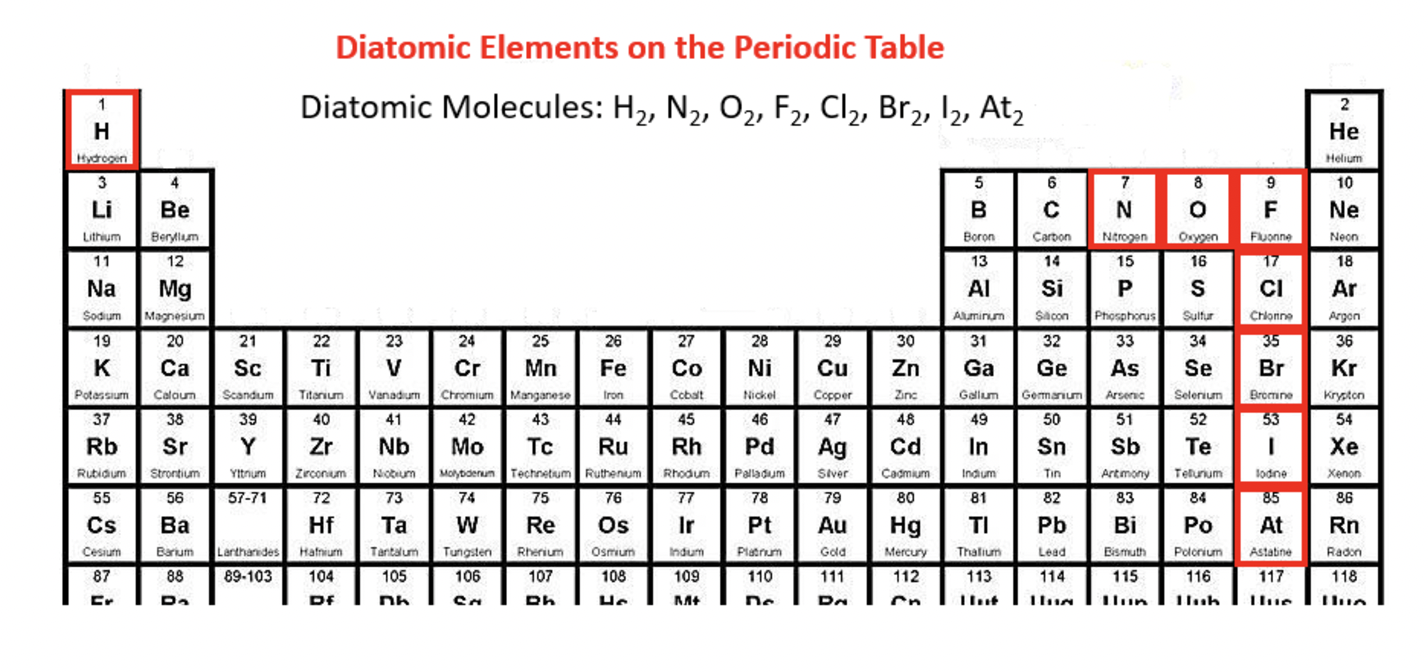
\includegraphics[width=1\linewidth]{diatomics.png}
    \label{fig:y}
\end{figure}

\subsection{Balancing Chemical Equations and Stoichiometry}

\textbf{Rules and Guidelines (red = rule):}

\begin{enumerate}[leftmargin=*, nosep]
    \item \textcolor{red}{At the end, there should be the same number of each element on  both sides. (conservation of matter)*}
    \item \textcolor{red}{Only balance after all compounds are written correctly. (ionic compounds are charge balanced)}
    \item \textcolor{red}{The lowest whole-number ratio of coefficients is used.} 
    \item Work left to right.
    \item Balance lone elements last.
    \item ``1" is not needed as a coefficient.
    \item Working back and forth may be necessary.
    \item If a polyatomic ion is present on both sides, balance as a single unit.
\end{enumerate}
\vspace{1em}
Example: \textcolor{blue}{Calcium hydroxide} reacts with \textcolor{blue}{sodium phosphate} to form \textcolor{blue}{sodium hydroxide} and \textcolor{blue}{calcium phosphate}. How many grams of \textcolor{blue}{sodium hydroxide} will be produced from \textcolor{blue}{18.4 grams of sodium phosphate?}

\textcolor{blue}{\textbf{Step 1:} Balance the ionic compounds} and write out the equation.
$$\text{Ca(OH)}_2 + \text{Na}_3\text{PO}_4 \longrightarrow \text{NaOH} +  \text{Ca}_3(\text{PO}_4)_2$$

\textcolor{blue}{\textbf{Step 2:} Balance the equation} using the rules and guidelines above.
$$\text{3Ca(OH)}_2 + \text{2Na}_3\text{PO}_4 \longrightarrow \text{6NaOH} +  \text{Ca}_3(\text{PO}_4)_2$$

\textcolor{blue}{\textbf{Step 3:} Draw a conversion map} from grams of sodium phosphate to grams of sodium hydroxide.
$$g \: \text{Na}_3\text{PO}_4 \longrightarrow mol \: \text{Na}_3\text{PO}_4 \longrightarrow mol \: {\text{NaOH}} \longrightarrow g \: {\text{NaOH}}$$

\textcolor{blue}{\textbf{Step 4:} Set up the equation.} 
$$(18.4 \: g \: \text{Na}_3\text{PO}_4) \times \left(\frac{1 \: mol \: \text{Na}_3\text{PO}_4}{163.94 \: g \: \text{Na}_3\text{PO}_4}\right) \times \left(\frac{3 \: mol \: \text{NaOH}}{1 \: mol \: \text{Na}_3\text{PO}_4}\right) \times \left(\frac{39.997 \: g \: \text{NaOH}}{1 \: mol \: \text{NaOH}}\right) $$
The third fraction (going from moles of sodium phosphate to moles of sodium hydroxide) is the \textbf{molar ratio}, found from the balanced equation. The original ratio is 6:2, which is simplified to 3:1.

\textcolor{blue}{\textbf{Step 4:} Calculate.} 
$$= \boxed{13.467 \: g \: \text{NaOH}}$$

\end{document}